\chapter{OpenGrok}
\label{chap:opengrok}

\section{Overview}
\label{opengrok_overview}
OpenGrok is an open-source search engine written in
Java\footnote{\url{https://en.wikipedia.org/wiki/Java\_(programming\_language)}}
freely available at \url{https://github.com/oracle/opengrok} under CDDL
license\footnote{\url{https://en.wikipedia.org/wiki/Common\_Development\_and\_Distribution\_License}}.
However, OpenGrok is different to most of the search engines, purpose of which is to traverse web and find the most relevant
webpages. OpenGrok provides searching across codebases. For instance, if you would like to know which files are using
\textit{mmap} function in \textit{Linux kernel}\footnote{\url{https://en.wikipedia.org/wiki/Linux\_kernel}} then
OpenGrok is the tool for that purpose. It understands a variety of
programming languages, e.g. Java, C, C\#, JavaScript and many others. The code analysis is done by
Ctags\footnote{\url{https://en.wikipedia.org/wiki/Ctags}}.
The other most notable features of OpenGrok are:
\begin{itemize}
    \item Support for multiple projects.
    \item Support for authentization and authorization (\cite{OpengrokAuthLayer}). For instance, by using LDAP
        \footnote{\url{https://en.wikipedia.org/wiki/Lightweight_Directory_Access_Protocol}}.
    \item Support for multiple version control systems\footnote{\url{https://en.wikipedia.org/wiki/Version\_control}},
        e.g. git, mercurial, etc.
        \begin{itemize}
            \item Support for searching in the repository history.
            \item Possibility to annotate a file.
            \item Possibility to see the history for a specific file.
        \end{itemize}
    \item Support for cross-referencing.
    \item Support for navigation in source files. For instance, by providing list of methods.
    \item Syntax highlighting of source files.
\end{itemize}

\section{Modules}
\label{opengrok_modules}

OpenGrok is split into multiple modules:
\begin{itemize}
    \item jrcs – Java library which provides support for RCS\footnote{\url{https://en.wikipedia.org/wiki/Revision\_Control\_System}}
    version control system.
    \item Indexer – described in \ref{indexer}.
    \item Web – described in \ref{opengrok-web}.
    \item plugins – contains authorization plugins.
    \item distribution – does not contain any code and serves for combining all of the above into one distribution unit.
\end{itemize}

Visualization of these modules and how they are dependent on each other can be seen in Figure \ref{opengrok_modules_img}.
\begin{figure}[htbp]
\centering
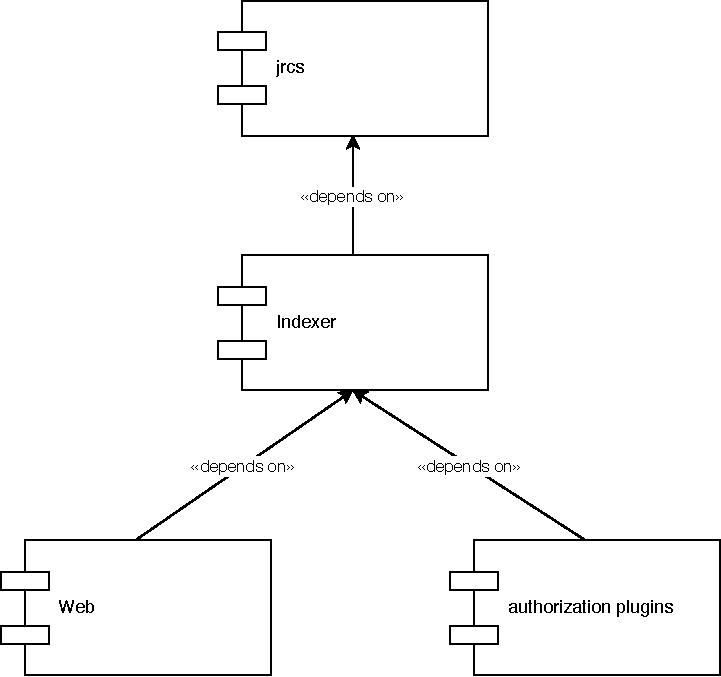
\includegraphics[width=100mm]{../img/opengrok_modules.pdf}
\caption{OpenGrok modules}
\label{opengrok_modules_img}
\end{figure}

Multiple-module support in one project is achieved by Maven\footnote{\url{https://maven.apache.org}} build tool.
There is one main \textit{pom.xml} in the root of the project which aggregates all the modules.

\subsection{Indexer}
\label{indexer}

Indexer is a submodule, main purpose of which is for each project to:
\begin{itemize}
    \item Generate the main lookup index. Detailed description in \ref{indexer:index}.
    \item Generate the history index for repositories. Detailed description in \ref{indexer:history}.
    \item Generate xref. Detailed description in \ref{indexer:xref}.
\end{itemize}

\subsubsection{Index}
\label{indexer:index}

OpenGrok heavily relies on Apache Lucene\footnote{\url{https://lucene.apache.org}} \citep{lucene_in_action}, a search engine library
written in Java. Every source file is considered to be a \textit{document}. Every \textit{document} has multiple
\textit{field}s which contain text data. This text data is then tokenized by specific rules (e.g. remove stop words,
stemming, etc.) into tokens. In the Lucene context \textit{term} is a pair of \textit{field} and \textit{token}.
Lucene uses \textit{reverse document index}\footnote{\url{https://en.wikipedia.org/wiki/Inverted_index}},
i.e. for each term a collection of document identifiers is stored in which this term occurrs.
This form of data representation is very efficient for document lookup.

\paragraph{Tokenization}
% TODO: should be here?

\paragraph{Lucene Internals}
% TODO: rewrite this? http://lucene.apache.org/core/7_3_1/core/org/apache/lucene/codecs/lucene50/Lucene50PostingsFormat.html

\subsubsection{History}
\label{indexer:history}

OpenGrok uses the history index for quick access to history information of every file in a project. OpenGrok first discovers
what kind of version control system the project is using and then executes appropriate commands to retrieve the project's
history (e.g. some form of \textit{git log}). Since executing these commands is not very efficient (new process has to
be created), OpenGrok does this at the indexing phase to provide better performance later. Serialized form of Java object
is stored for each source file of the project to represent its history.

\subsubsection{Xref}
\label{indexer:xref}

Main purpose of the OpenGrok is to find relevant documents based on the search query. After the successful search, the most
obvious route of action is to look at the found documents. However, analyzing the document once again, performing syntax
highlighting and other operations can be very time consuming. Therefore, \textit{xref} directory contains pre-generated
HTML\footnote{\url{https://en.wikipedia.org/wiki/HTML}} versions of every source file which already contain the
aforementioned information.

\subsection{Web}
\label{opengrok-web}

The previous section \ref{indexer:index} describes how the data are processed to create the index. However, these data need
to be presented to the end user. The Web submodule serves exactly this purpose. It is distributed as a
WAR\footnote{\url{https://en.wikipedia.org/wiki/WAR\_(file\_format)}} which can be used by many
servlet containers\footnote{\url{https://en.wikipedia.org/wiki/Web\_container}}. OpenGrok correctly runs in
Apache Tomcat\footnote{\url{http://tomcat.apache.org}}; nevertheless, there is no Tomcat vendor lock-in; therefore,
other servlet containers should work properly as well.

\subsubsection{Configuration}
\label{opengrok_configuration}

Since OpenGrok has two modules (Indexer and Web) which can be run separately, it needs a way to pass relevant
information between those. However, it might be possible that Indexer finishes its work after a long period of time
(in some cases it might take days) and the Web module is not reachable. Therefore, to not lose all of the information
needed by the Web module, the Indexer stores it in a configuration file. It is stored as an
XML\footnote{\url{https://en.wikipedia.org/wiki/XML}} encoded class which needs to be read by Web on its startup.
If the Web module does not find the configuration at the expected place (can be configured in \textit{web.xml}) then an
error is shown on the main page and the usage is not possible. Of course, there are ways to change the configuration
of the running OpenGrok application via the REST API \footnote{\url{https://en.wikipedia.org/wiki/Representational\_state\_transfer}}
described in the \ref{opengrok_rest}.

\subsubsection{REST API}
\label{opengrok_rest}

Opengrok provides REST API support. This is a relatively new feature. Before that, OpenGrok had known a concept of
\textit{Messages} – custom serialization of Java objects passed to the Web application via a custom port.
So far, most of the REST API calls can be only made from the machine on which the OpenGrok runs.
This is mainly because these REST API calls are meant as a means of communication between the Indexer and Web application
or for administrators maintaining the OpenGrok instance. More information can be found at
\url{https://github.com/oracle/opengrok/wiki/Web-services}.

\section{Usage}
\label{opengrok_usage}
The main purpose of the OpenGrok project is to provide ability to search codebases of software projects. This is done
mainly through its web interface. The main OpenGrok page can be seen in the Figure \ref{opengrok_main}.

\begin{figure}[htbp]
    \centering
    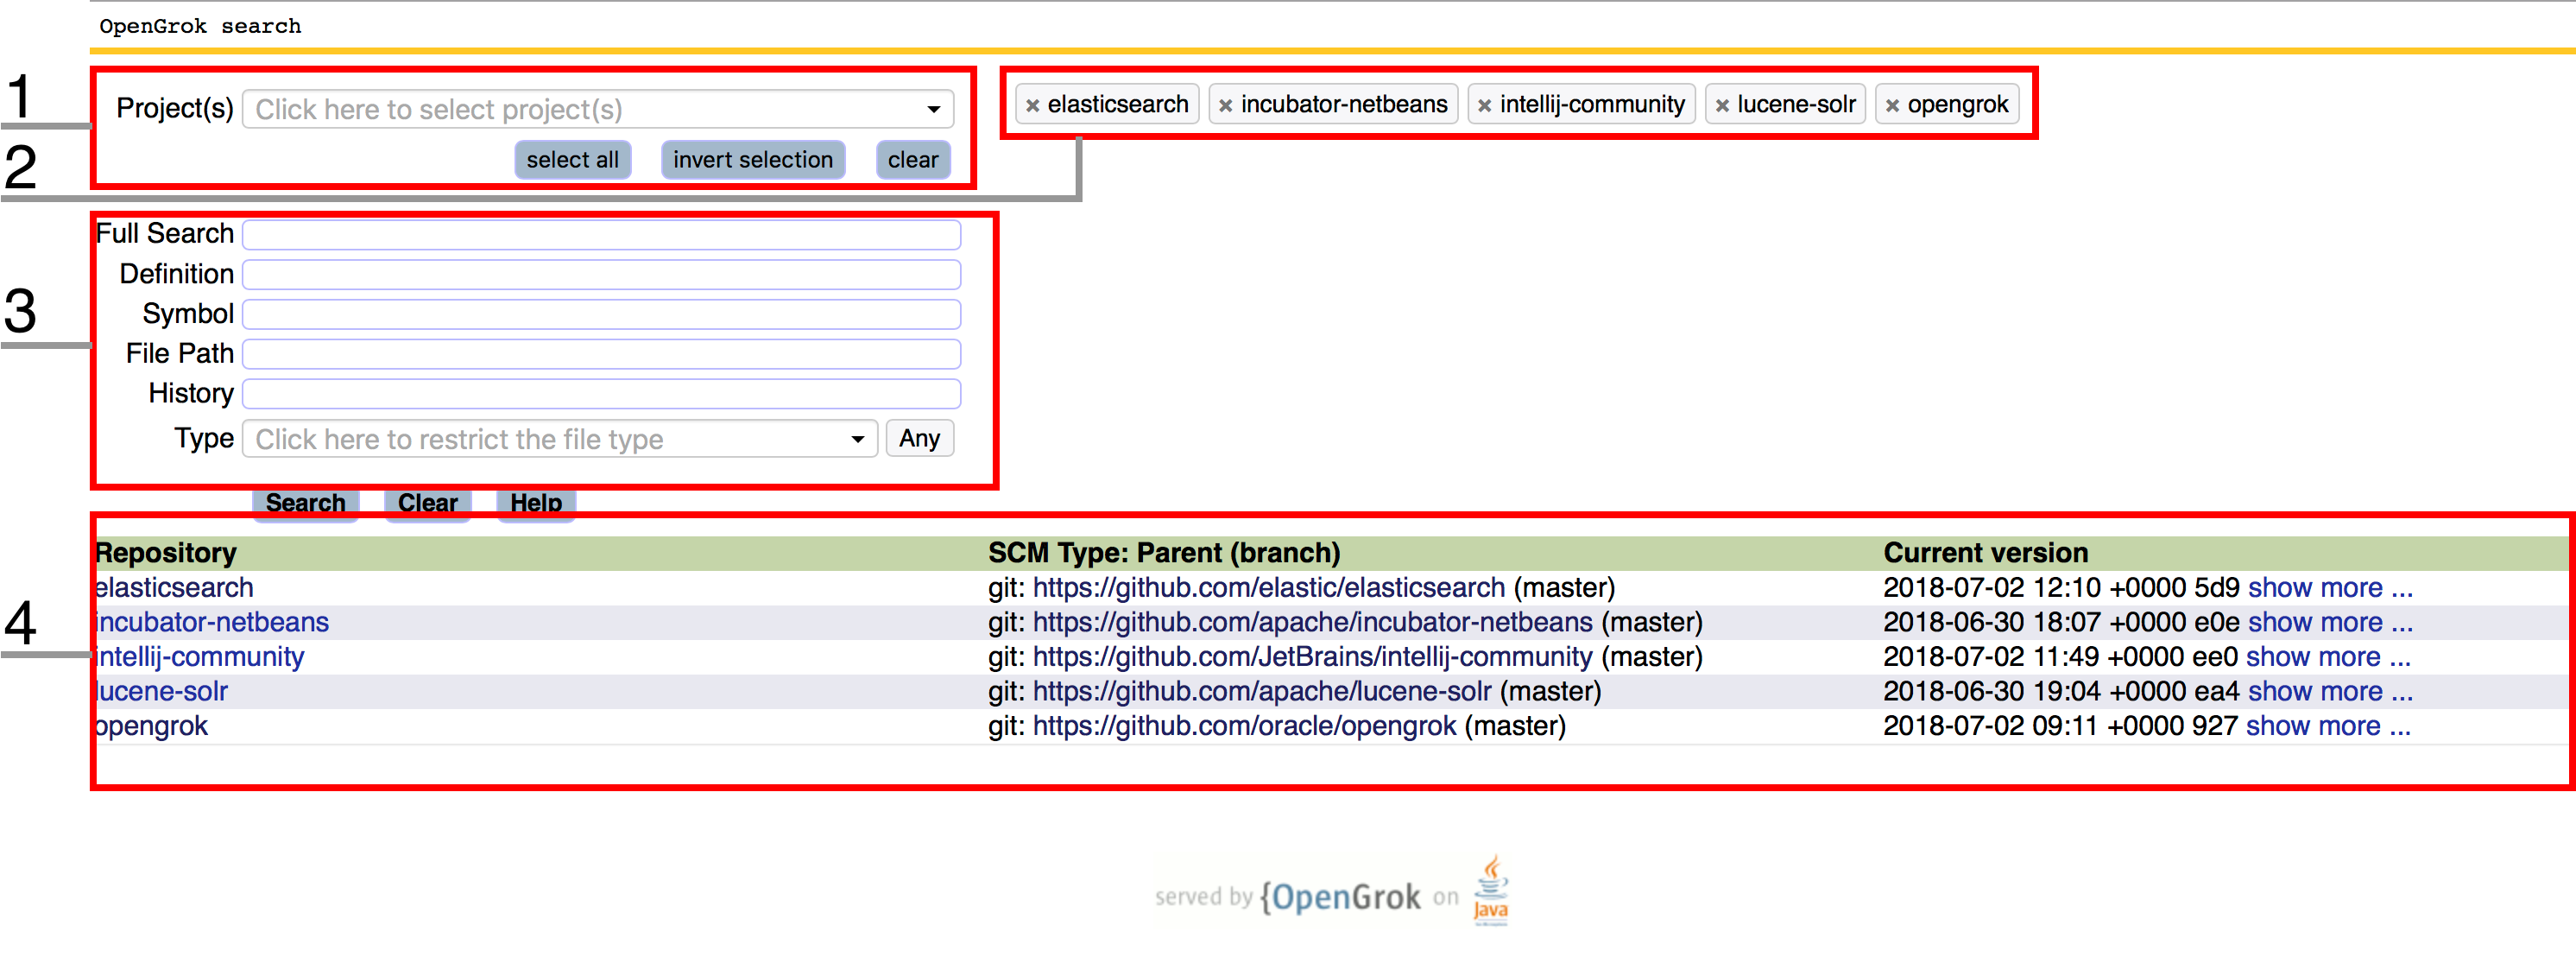
\includegraphics[width=145mm]{../img/opengrok_main.png}
    \caption{Main OpenGrok page}
    \label{opengrok_main}
\end{figure}

The numbers in the Figure \ref{opengrok_main} signify:
\begin{enumerate}
    \item Field where projects can be selected.
    \item Selected projects.
    \item Search fields.
       \begin{itemize}
        \item \textbf{Full search} – specifies the text the document should contain. Represents \textit{full} field in
        underlying Lucene implementation.
        \item \textbf{Definition} – specifies the definition of a symbol the document should contain.
        Represents \textit{defs} field in the underlying Lucene implementation.
        \item \textbf{Symbol} – specifies the symbol the document should contain.
        Represents \textit{refs} field in the underlying Lucene implementation.
        \item \textbf{File Path} – specifies the path the document should possess.
        Represents \textit{path} field in the underlying Lucene implementation.
        \item \textbf{History} – specifies the history the document should possess.
        Represents \textit{hist} field in the underlying Lucene implementation.
        \item \textbf{Type} – restricts the search for documents of the type.
        Represents \textit{type} field in the underlying Lucene implementation.
       \end{itemize}
    \item Repository list.
\end{enumerate}

It is possible to add values to multiple search fields to make the search more specific. Furthermore, any query written
in Lucene syntax can be typed into the search fields.

More detailed information with examples can be found on the \textit{/help.jsp} web page of the running OpenGrok Web application instance.

\subsection{Navigating Results}

OpenGrok presents search results similarly to what can be seen in Figure \ref{opengrok_results}.

\begin{figure}[htbp]
    \centering
    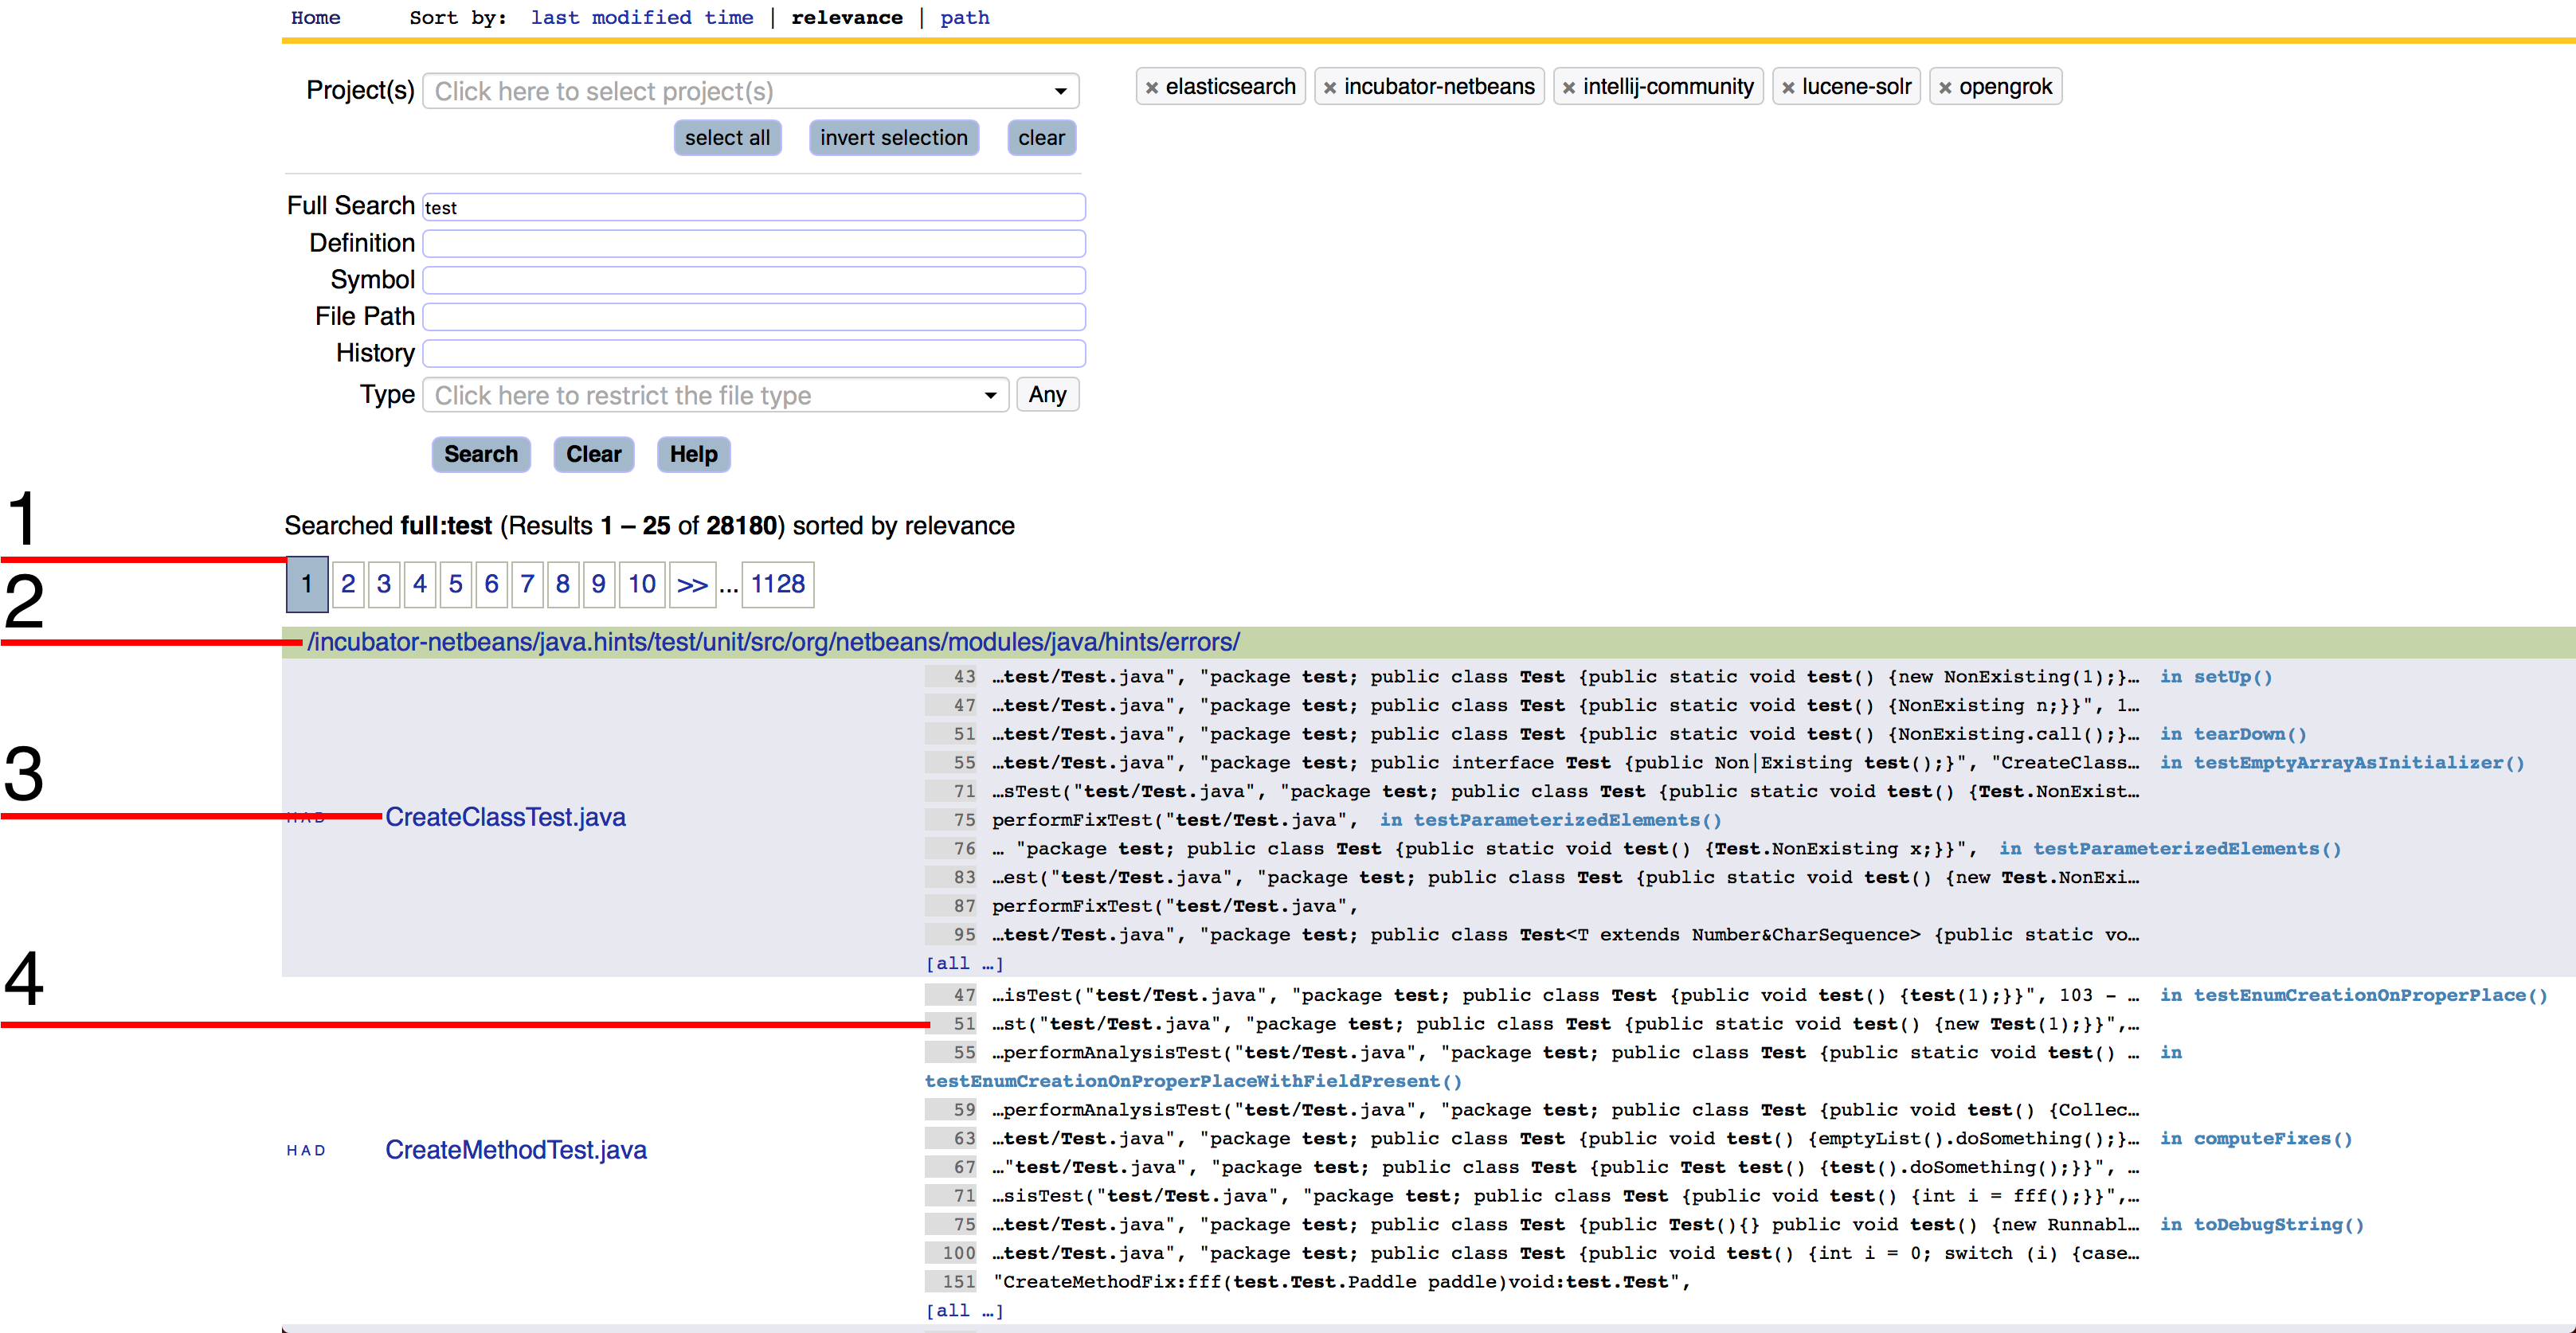
\includegraphics[width=145mm]{../img/opengrok_results.png}
    \caption{OpenGrok search results}
    \label{opengrok_results}
\end{figure}

In the picture \ref{opengrok_results} numbers represent:
\begin{enumerate}
    \item Results are paged as is a custom in many applications.
    \item Directory where the result documents are located.
    \item Document that satisfies the search criteria.
    \item Line number and content of the line where the match was found.
\end{enumerate}

\subsection{Traversing Source Code}

OpenGrok presents files' content similarly to modern
IDEs\footnote{\url{https://en.wikipedia.org/wiki/Integrated_development_environment}}. This can be noticed in the Figure
\ref{opengrok_source} where numbers represent:

\begin{enumerate}
    \item Line numbers.
    \item File content.
    \item Current code scope of the content that is displayed.
    \item Window with quick navigation links across the source file.
\end{enumerate}

\begin{figure}[htbp]
    \centering
    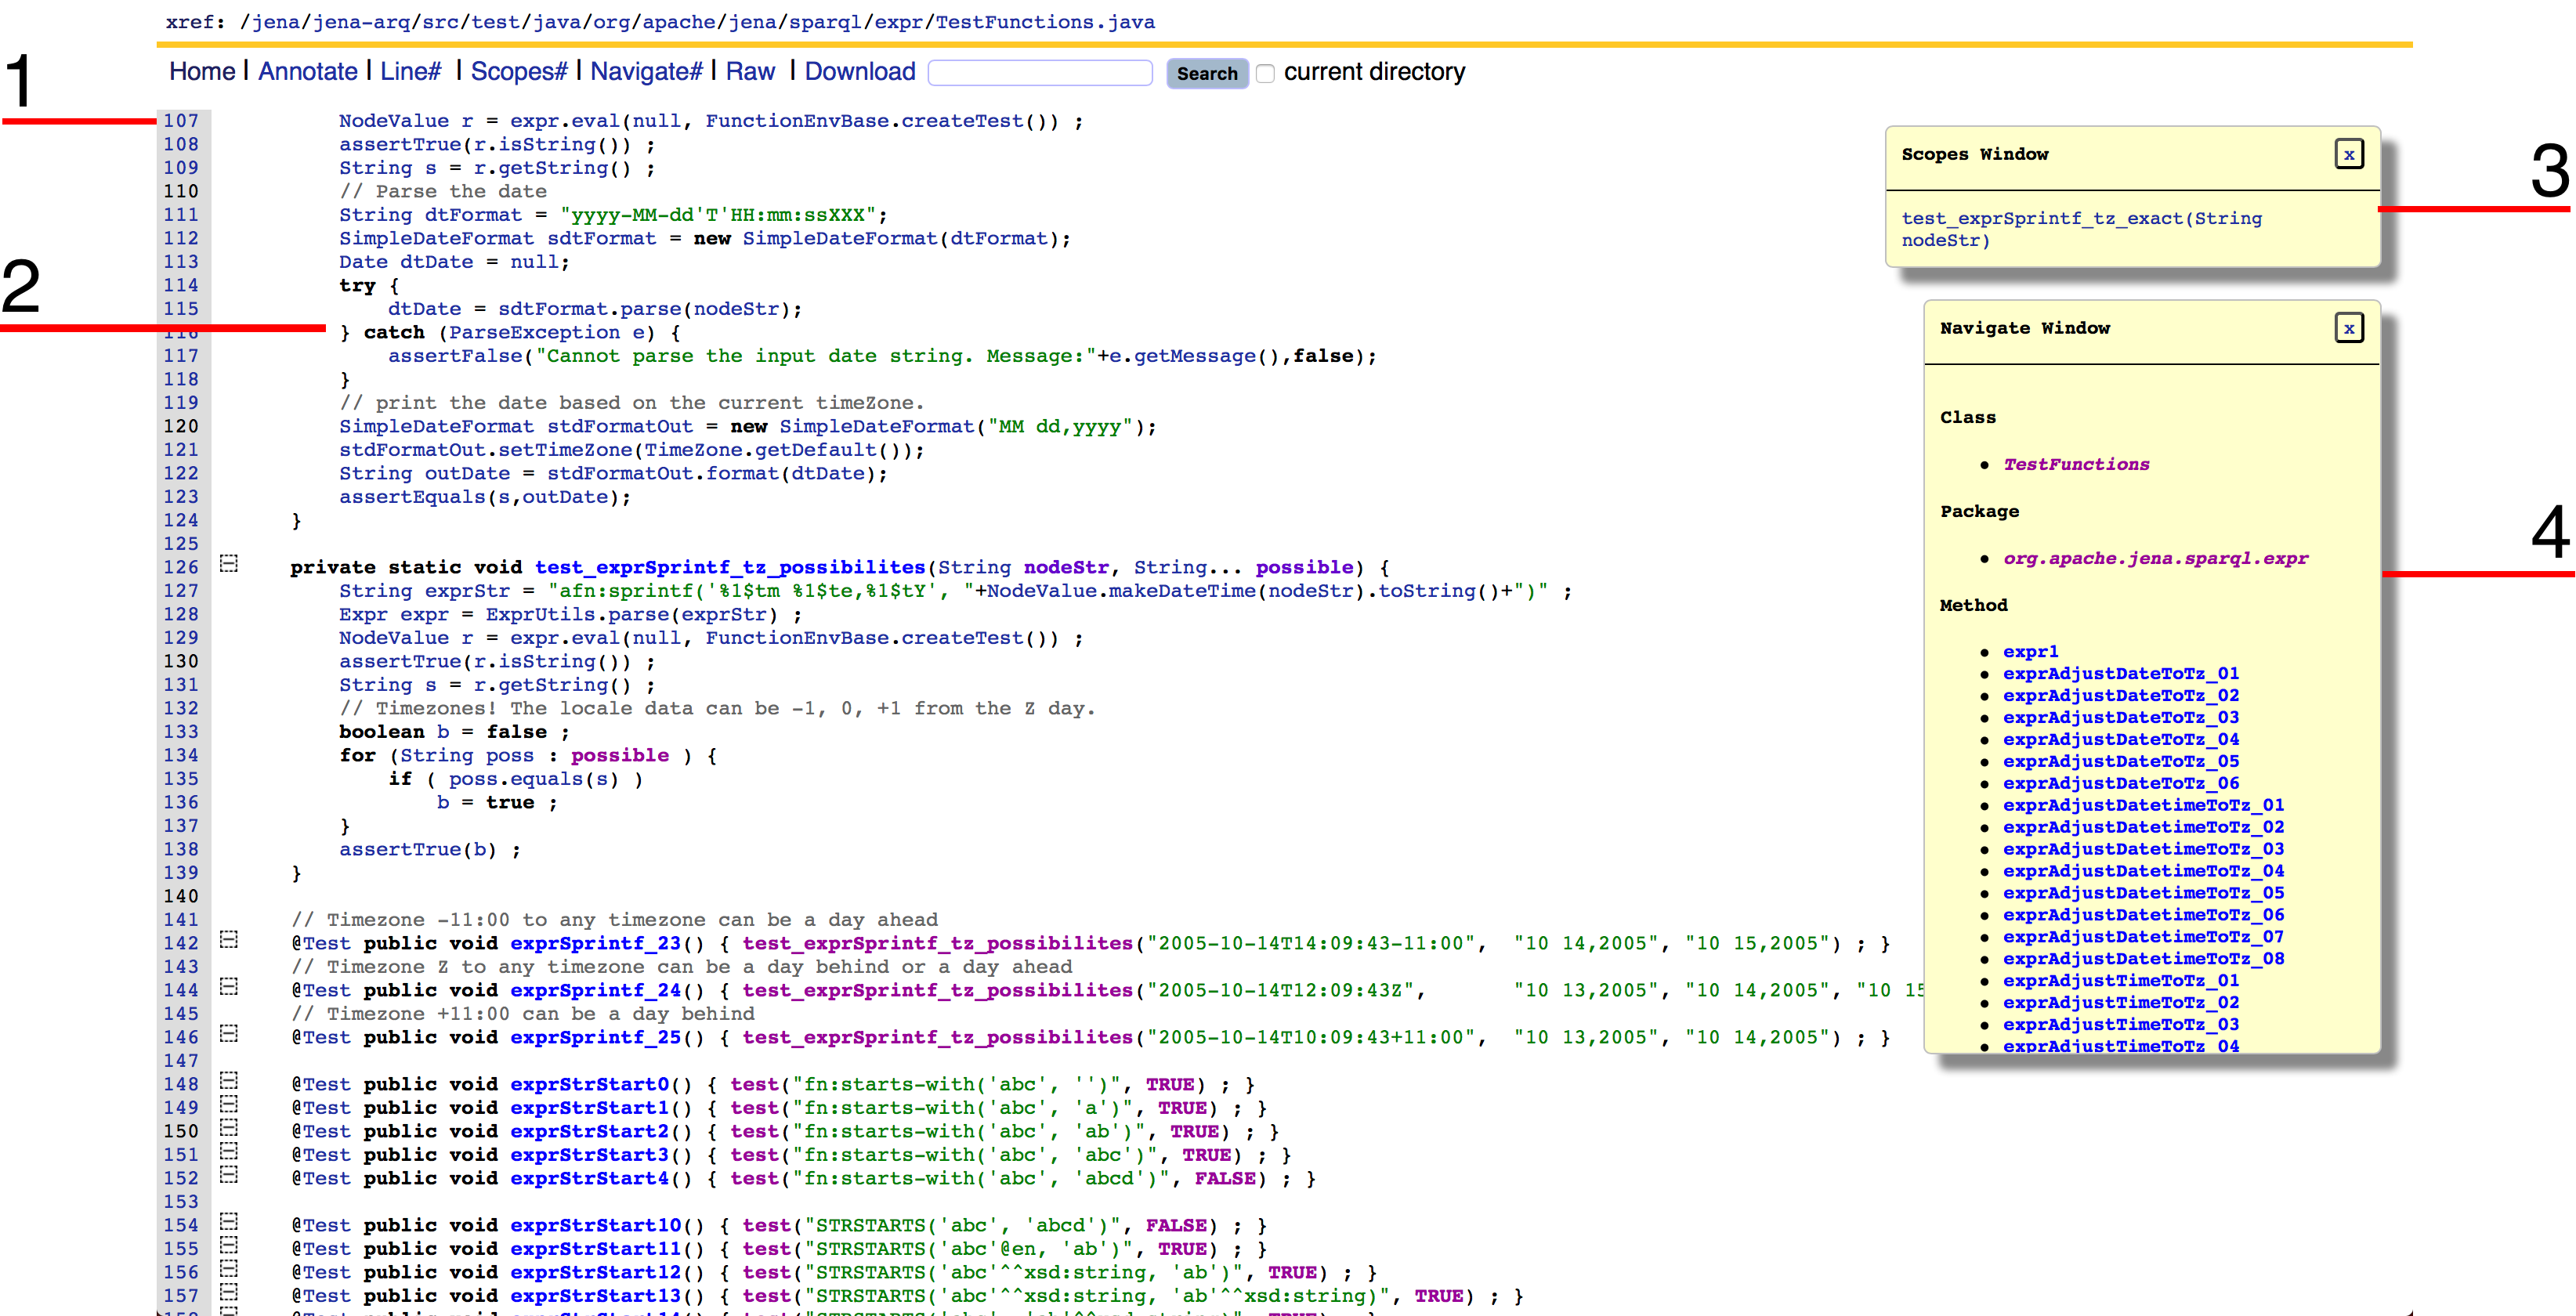
\includegraphics[width=145mm]{../img/opengrok_source.png}
    \caption{OpenGrok file content}
    \label{opengrok_source}
\end{figure}

\section{Similar Tools}
It is hard to compare OpenGrok to other similar tools because all of these are complex and each of them provides a unique
feel and solution to the problems.
Therefore, the list only mentions if these tools contain suggester functionality. Still, this might not be the best
indicator because they might provide different solutions, e.g. instant search which might render the suggester a redundant asset.
The list of similar tools:
\begin{itemize}
    \item \textbf{SourceGraph} \url{https://about.sourcegraph.com} – SourceGraph supports the instant search feature.
    While typing some text into the search field, it immediately displays the files in which the text has been found. The Figure
    \ref{sourcegraph} shows how this feature looks like.

    \begin{figure}[htbp]
        \centering
        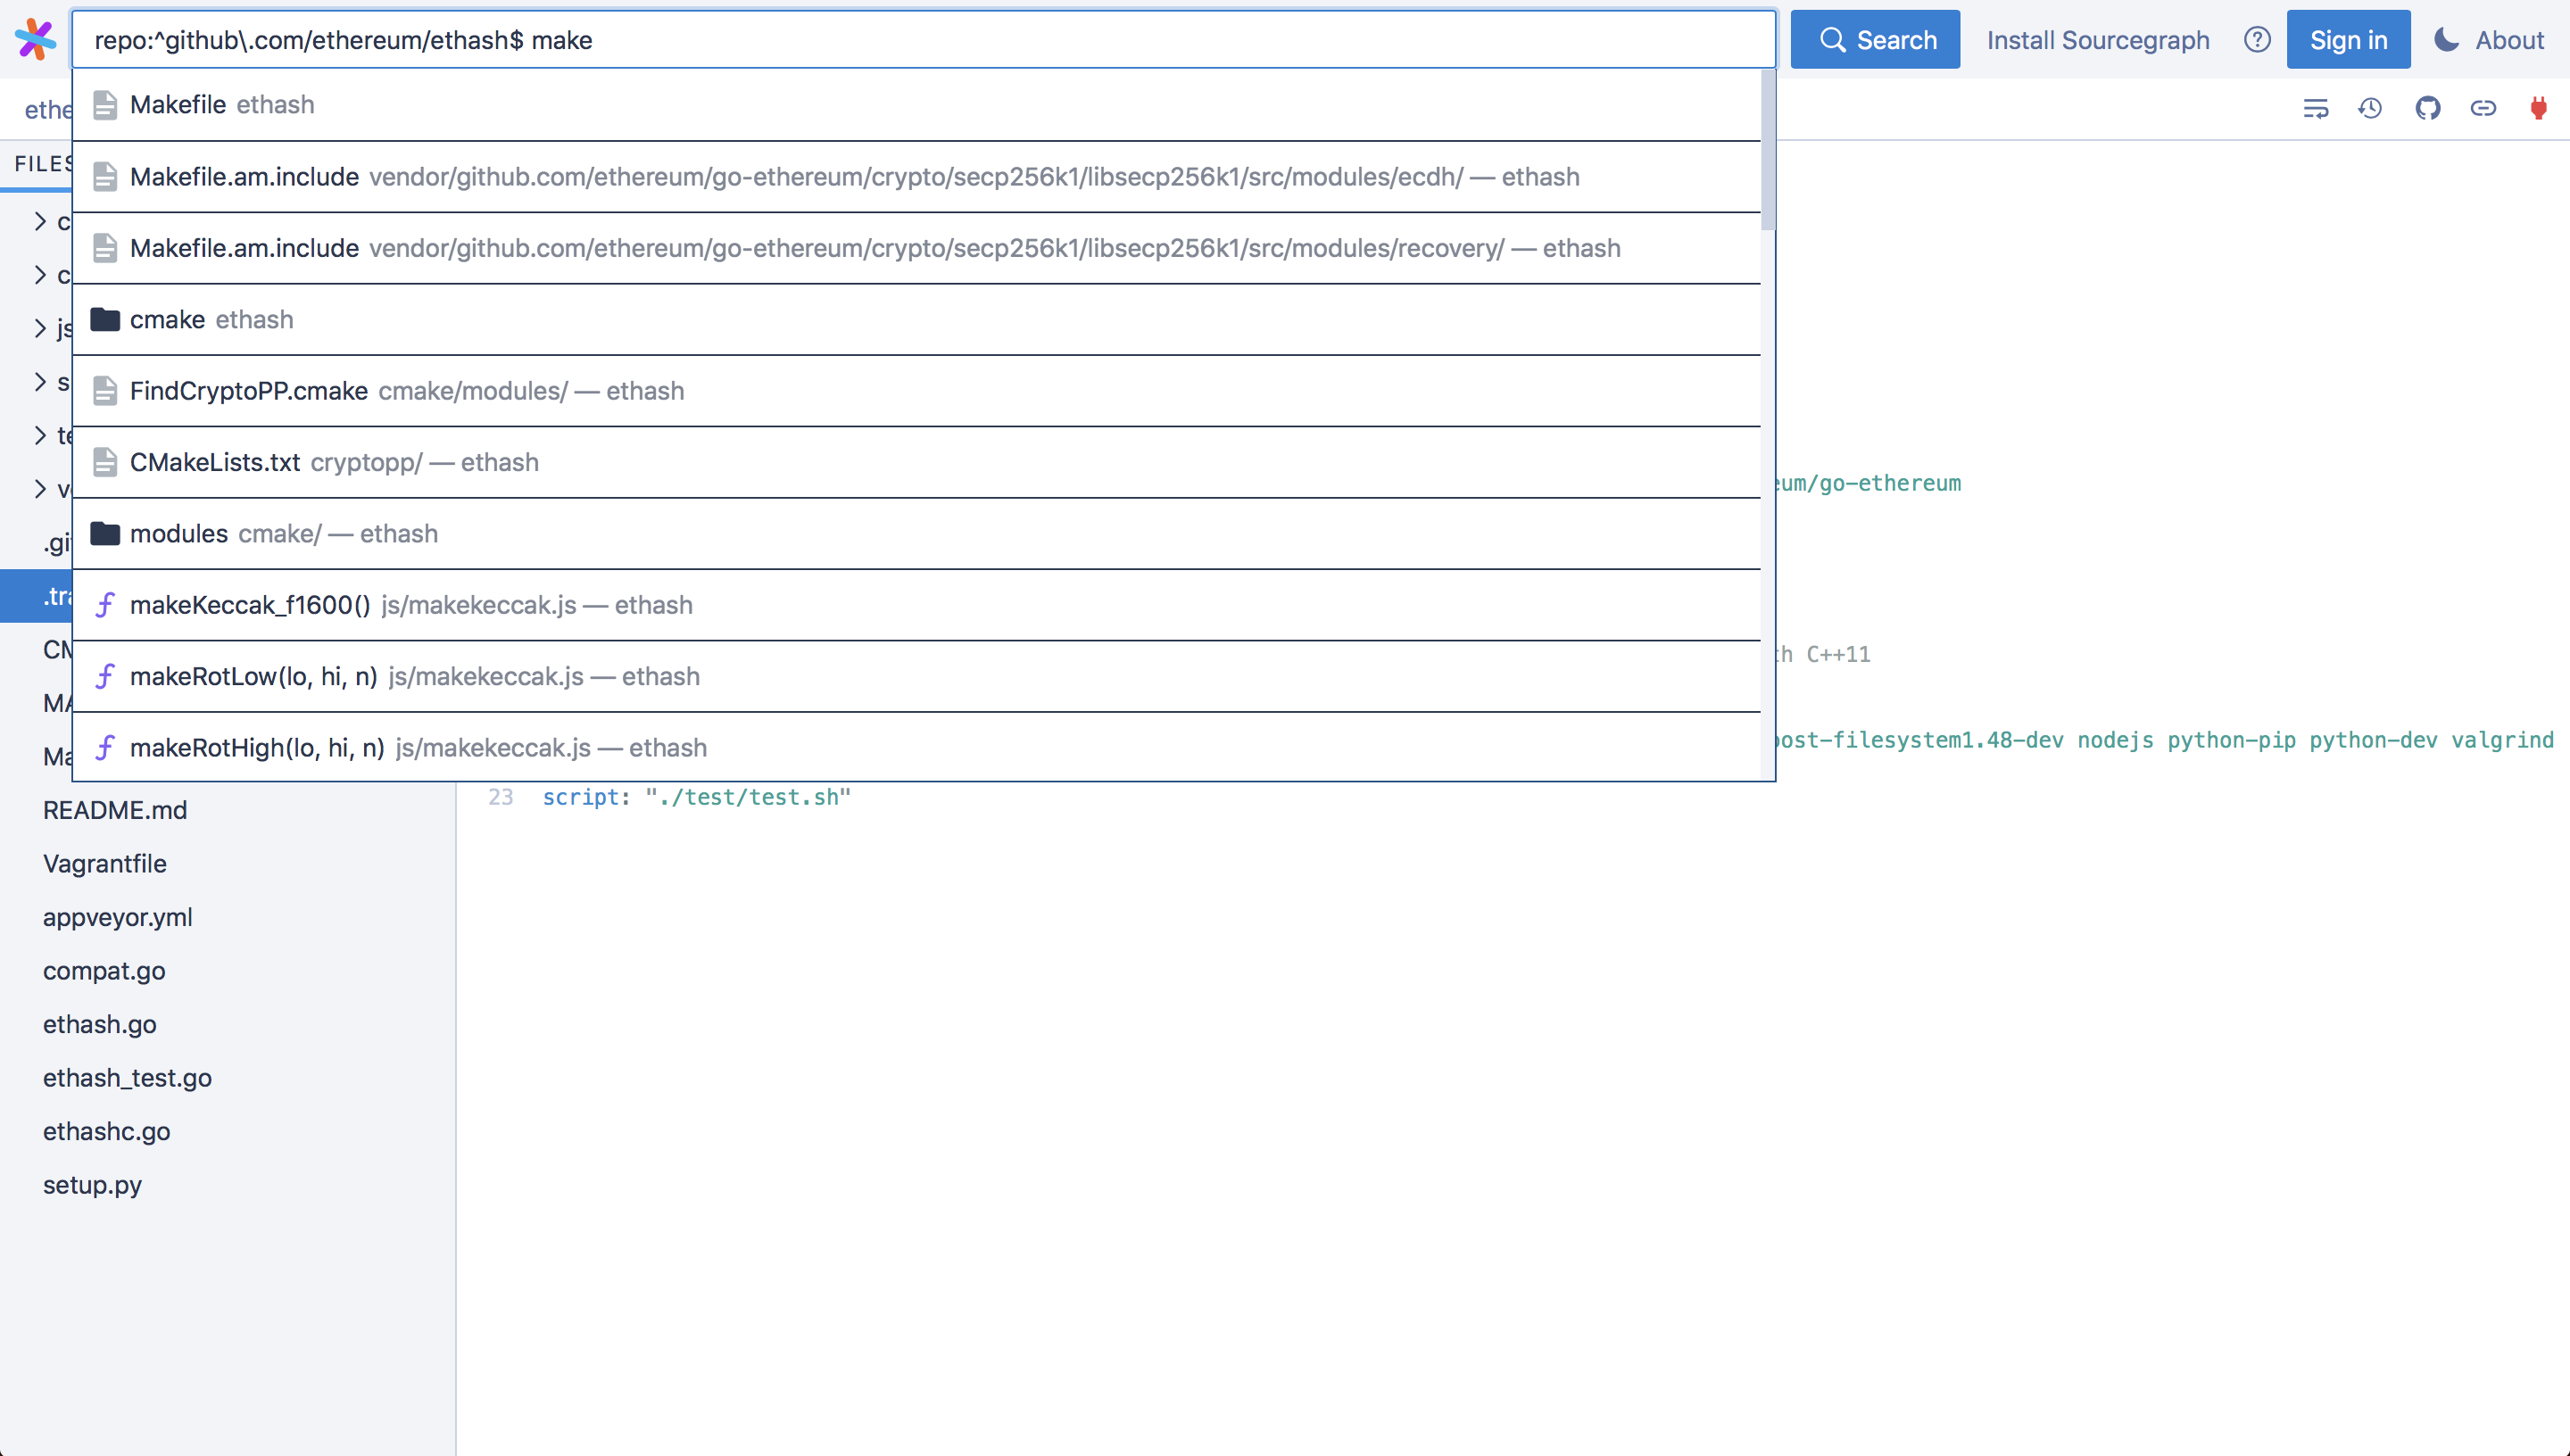
\includegraphics[width=145mm]{../img/sourcegraph.png}
        \caption{SourceGraph instant search feature}
        \label{sourcegraph}
    \end{figure}

    \item \textbf{searchcode} \url{https://searchcode.com/} – it seems that searchcode does not support neither
    autocomplete nor instant search feature.

    \item \textbf{livegrep} \url{https://livegrep.com/} – supports instant search. Immediately shows files and their contents
    where the text has been found. The look of this application can be seen in Figure \ref{livegrep}.

    \begin{figure}[htbp]
        \centering
        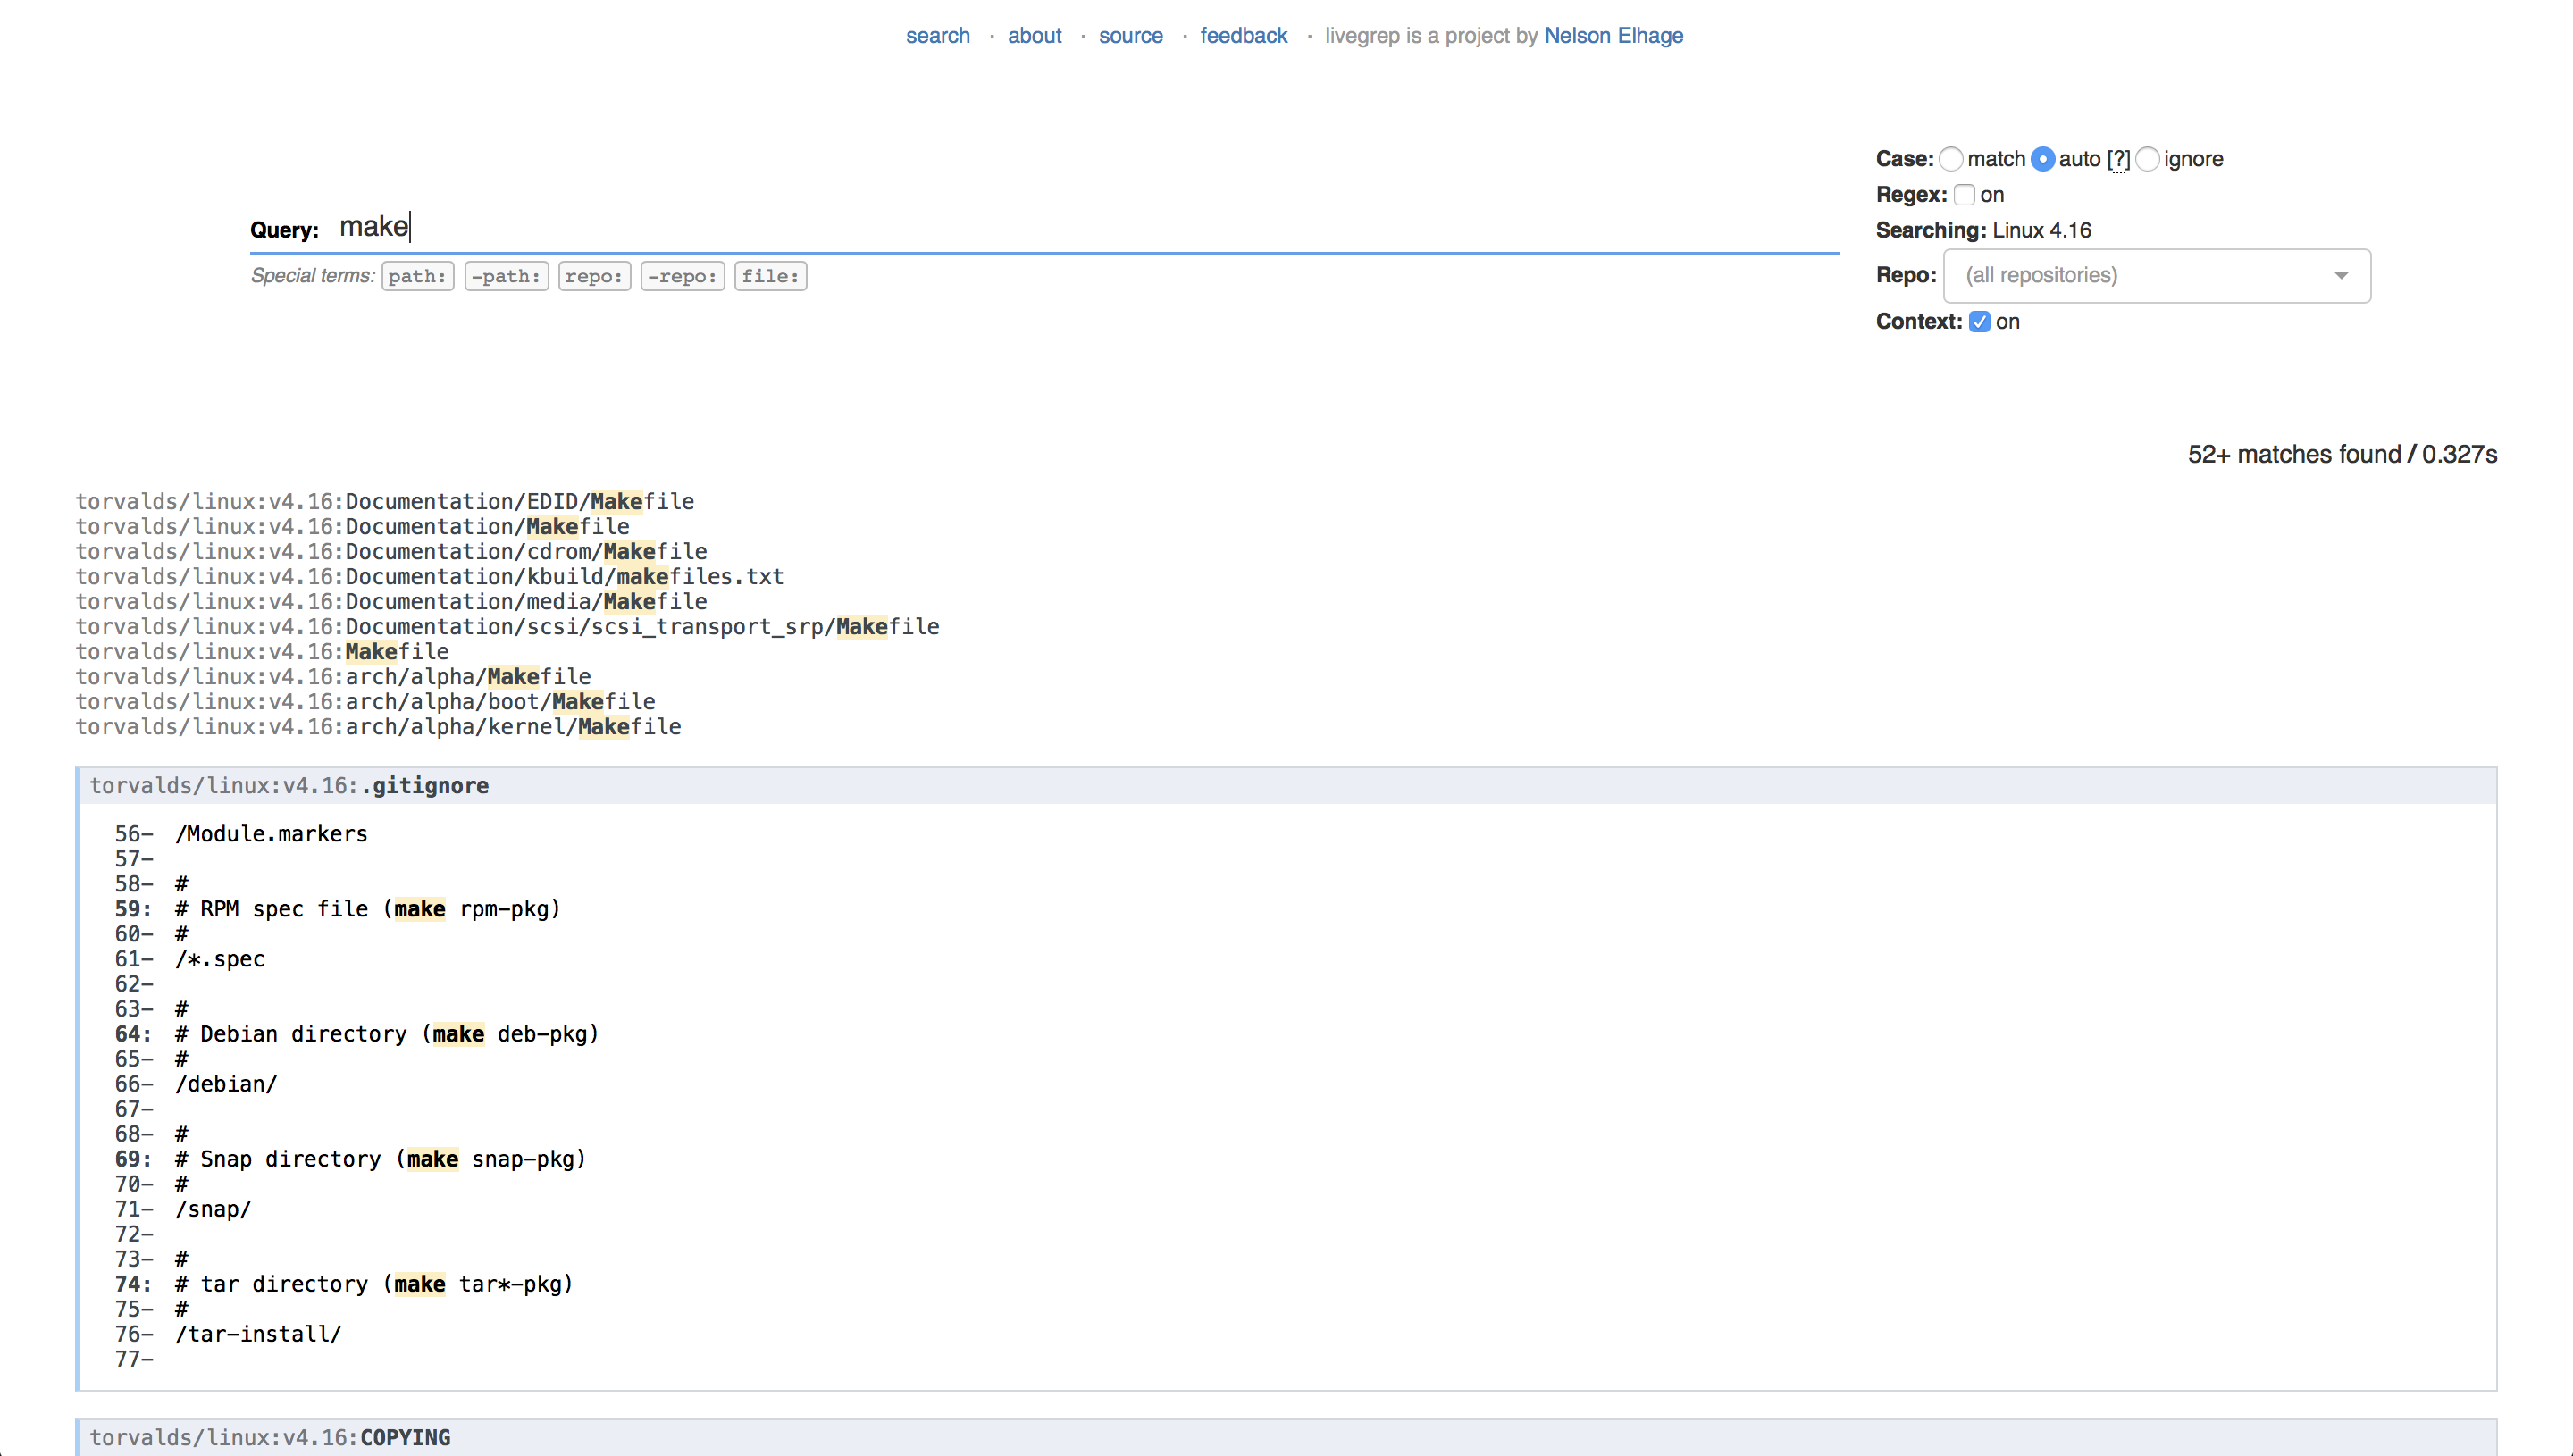
\includegraphics[width=145mm]{../img/livegrep.png}
        \caption{livegrep instant search feature}
        \label{livegrep}
    \end{figure}

    \item \textbf{Debian Code Search} – does not seem to have any suggester support. It was created as a
    bachelor thesis \citep{debian_search}. It searches all the open source projects which are included in the Debian archive.
    The search is based on the article \citep{russ_cox} which explains how Google Code Search worked.

\end{itemize}
